\documentclass[draft=false,paper=a4,twoside=false,fontsize=11pt,headsepline,BCOR10mm,DIV11,liststotoc]{scrbook}
% \usepackage{showframe}
\usepackage{titlesec}
% \def\chaptertitlename{Section}
% \titleformat{\chapter}{\normalfont\Large\bfseries}{\chaptertitlename\ \thechapter{:\ }}{0pt}{\Large}{}
\titleformat{\chapter}[hang]{\huge\bfseries}{\thechapter\quad}{0pt}{}
% \titlespacing{\chapter}{0pt}{-20pt}{30pt}
\titlespacing{\chapter}{0pt}{-3em}{2em}
\usepackage[ngerman,english]{babel}
\usepackage[latin1]{inputenc}
\usepackage[babel,german=quotes]{csquotes}
%% see http://www.tex.ac.uk/cgi-bin/texfaq2html?label=uselmfonts
\usepackage[T1]{fontenc}
%\usepackage[utf8]{inputenc}
\usepackage{eurosym}
\usepackage{libertine}
\usepackage{pifont}
\usepackage{microtype}
\usepackage{textcomp}
% \usepackage[intoc,german,prefix]{nomencl}
\usepackage{setspace}
\usepackage{makeidx}
\usepackage{listings}
\usepackage{natbib}
\usepackage[ngerman,colorlinks=true]{hyperref}
\usepackage{soul}
\usepackage{tabularx}
\usepackage{multirow}
\usepackage{multicol}
\usepackage{glossaries}
%%\usepackage{booktabs}
\usepackage{colortbl}
\usepackage[final]{pdfpages}
\usepackage[printer]{hawstyle}
% \usepackage{hawstyle}
\usepackage{caption}
\usepackage{lipsum} %% for sample text

\usepackage{float}
\restylefloat{table}
\restylefloat{figure}


\definecolor{middlegray}{rgb}{0.5,0.5,0.5}
\definecolor{lightgray}{rgb}{0.8,0.8,0.8}

%% define some colors
\colorlet{BackgroundColor}{gray!20}
\colorlet{KeywordColor}{blue}
\colorlet{CommentColor}{black!60}
%% for tables
\colorlet{HeadColor}{gray!60}
\colorlet{Color1}{blue!10}
\colorlet{Color2}{white}

%% configure colors
\HAWifprinter{
  \colorlet{BackgroundColor}{gray!20}
  \colorlet{KeywordColor}{black}
  \colorlet{CommentColor}{gray}
  % for tables
  \colorlet{HeadColor}{gray!60}
  \colorlet{Color1}{gray!40}
  \colorlet{Color2}{white}
}{}
\lstset{%
  language=JAVA,
  numbers=left,
  numberstyle=\tiny,
  stepnumber=1,
  tabsize=2,
  numbersep=-10pt,
  basicstyle=\ttfamily\small,
  keywordstyle=\color{KeywordColor}\bfseries,
  identifierstyle=\color{black},
  commentstyle=\color{middlegray},
  backgroundcolor=\color{BackgroundColor},
  captionpos=b,
  breaklines=true,
  fontadjust=true,
  flexiblecolumns=true
}
\lstset{escapeinside={(*@}{@*)}, % used to enter latex code inside listings
        morekeywords={uint32_t, int32_t}
}

% \usepackage{courier}
% \usepackage{caption}
% \lstset{
%   basicstyle=\footnotesize\ttfamily, % Standardschrift
%   numbers=left,               % Ort der Zeilennummern
%   numberstyle=\tiny,          % Stil der Zeilennummern
%   %stepnumber=2,               % Abstand zwischen den Zeilennummern
%   numbersep=5pt,              % Abstand der Nummern zum Text
%   tabsize=2,                  % Groesse von Tabs
%   extendedchars=true,         %
%   breaklines=true,            % Zeilen werden Umgebrochen
%   keywordstyle=\color{red},
%   %frame=b,         
%   %        keywordstyle=[1]\textbf,    % Stil der Keywords
%   %        keywordstyle=[2]\textbf,    %
%   %        keywordstyle=[3]\textbf,    %
%   %        keywordstyle=[4]\textbf,   \sqrt{\sqrt{}} %
%   stringstyle=\color{white}\ttfamily, % Farbe der String
%   showspaces=false,           % Leerzeichen anzeigen ?
%   showtabs=false,             % Tabs anzeigen ?
%   xleftmargin=17pt,
%   framexleftmargin=17pt,
%   framexrightmargin=5pt,
%   framexbottommargin=4pt,
%   %backgroundcolor=\color{lightgray},
%   showstringspaces=false      % Leerzeichen in Strings anzeigen ?        
% }
% %\DeclareCaptionFont{blue}{\color{blue}} 
% 
% %\captionsetup[lstlisting]{singlelinecheck=false, labelfont={blue}, textfont={blue}}
% \DeclareCaptionFont{white}{\color{white}}
% \DeclareCaptionFormat{listing}{\colorbox{HeadColor}{\parbox{\textwidth}{\hspace{15pt}#1#2#3}}}
% \captionsetup[lstlisting]{format=listing,labelfont=white,textfont=white, singlelinecheck=false, margin=0pt, font={bf,footnotesize}}



\ifpdfoutput{
  \hypersetup{bookmarksopen=false,bookmarksnumbered,linktocpage}
}{}

%% more fancy C++
\DeclareRobustCommand{\cxx}{C\raisebox{0.25ex}{{\scriptsize +\kern-0.25ex +}}}

\clubpenalty=10000
\widowpenalty=10000
\displaywidowpenalty=10000

% unknown hyphenations
\hyphenation{
}

%% recalculate text area
\typearea[current]{last}

\makeindex
%% \makenomenclature
\makeglossaries

\begin{document}
\selectlanguage{ngerman}

%%%%%
%% customize (see readme.pdf for supported values)
\HAWThesisProperties{Author={Shirin Bediako \\ MatrNr.: 2088775 \\ shirin.bediako@haw-hamburg.de}
                    ,AuthorTwo={Jelka Dr�cker \\ MatrNr.:2079988 \\ jelka.dr�cker@haw-hamburg.de}
                    ,Title={Die bikulturelle Identit"atsentwicklung afrodeutscher Kinder}
                    ,SubTitle={Bikulturalit"at als Einflussfaktor auf die Identit"atsentwicklung afrodeutscher Kinder}
                    ,EnglishTitle={Die bikulturelle Identit"atsentwicklung afrodeutscher Kinder}
                    ,ThesisType={Hausarbeit}
                    ,ExaminationType={Einf�hrung in die Familienberatung}
                    ,DegreeProgramme={Bildung und Erziehung in der Kindheit}
                    ,ThesisExperts={Prof.\ Dr.\ Wolfgang\ Hantel-Quitmann}
                    ,ReleaseDate={17. Oktober 2013}
                  }

%% title
\frontmatter

%% output title page
\maketitle

\onehalfspacing

%% add abstract pages
%% note: this is one command on multiple lines
% \HAWAbstractPage
%% German abstract
% {keywords...}%
% {text...}
%% English abstract
% {keywords...}%
% {text...}

\newpage
\singlespacing

\tableofcontents
\newpage
%% enable if these lists should be shown on their own page
% \listoftables
\listoffigures
% \lstlistoflistings

%% main
\mainmatter
\onehalfspacing
\newglossaryentry{Bewegungsangebote}{name={Bewegungsangebote},description={Unter Bewegungsangeboten werden, Bewegungsm�glichkeiten verstanden, die vom p�dagogischen Fachpersonal gestellten werden. Hierunter fallen r�umliche Gegebenheiten, sowie die Materialien die die Kinder nutzen k�nnen. Die Kinder haben hier unter p�dagogisch Aufsicht, die M�glichkeit frei zu spielen. Freispiel in vorbereiteter Umgebung.}}

\newglossaryentry{Bewegungsspiele}{name={Bewegungsspiele},description={Als Bewegungsspiele werden Spiel bezeichnet, die Bewegungst�tigkeiten von Kindern beschreibt, die sich aus Spielsituationen ergeben und meist selbstgesteuert sind.}}

\newglossaryentry{Egozentrismus}{name={Egozentrismus}, description={Ist die Tendenz, die Welt aus der eigenen Perspektive zu sehen.}}

\newglossaryentry{Empathie}{name={Empathie}, description={Als Empathie oder auch Einf�hlungsverm�gen wird die F�higkeit verstanden, Gef�hle bei anderen wahrzunehmen und sich in Gef�hlslage der andere Person hineinzuversetzen. Des Weiteren setzt es voraus, dass die eigenen Gef�hle von denen des anderen unterschieden werden. Empathie ist nicht zu verwechseln mit Gef�hlsansteckung oder Mitleid. Die F�higkeit empathisch zu denken, handeln und zu reagieren, k�nnen Kinder erst ausbilden, wenn sich das Selbstkonzept herausgebildet hat. Dieses erm�glicht die getrennte Wahrnehmung von dem \enquote{ich} und dem \enquote{anderen}.}}

\newglossaryentry{Freispiel}{name={Freispiel}, description={Das Freispiel ist ein wichtiger Bestandteil in der Tagesgestaltung im Kindergarten oder in der Kindertagesst�tte. Darunter wird verstanden,  Kindern die M�glichkeit zu bieten, w�hrend einer bestimmten Zeit, Spiele frei zu entwickeln und zu gestalten.}}

\newglossaryentry{Freundschaften}{name={Freundschaften}, description={Merkmal von Freundschaft ist die Freiwilligkeit, enge Gegegseitig positiv gesinnte Beziehung.}}

\newglossaryentry{Gleichaltrigen}{name={Gleichaltrigen}, description={siehe Peers}}

\newglossaryentry{Mitleid}{name={Mitleid}, description={Mitleid bezieht sich auf auf das Hineinversetzen in negative Gef�hle oder die Lebenslage einer anderen Person und dr�ckt sich in Anteilnahme, Kummer und Sorge aus.}}

\newglossaryentry{Peers}{name={Peers}, description={Peer sind Menschen von etwa gleichem Alter und Status.}}

\newglossaryentry{Prosoziales verhalten}{name={Prosoziales verhalten}, description={Das ist ein freiwilliges Verhalten, von denen andere einen positiven Effekt haben, wie zum Beispiel, jemanden zu tr�sten, etwas zu teilen oder zu helfen.}}

\newglossaryentry{soziometrischen Status}{name={soziometrischen Status}, description={Mit dem soziometrischer Status wird gemessen wie sehr ein Kind von seinen Peers als Gesamtgruppe gemocht wird.}}

\newglossaryentry{Selbstbild}{name={Selbstbild}, description={Das Selbstbild beschreibt das Bild, das sich ein Kind von seiner Person macht.}}

\newglossaryentry{Gefhlsansteckung}{name={Gef�hlsansteckung}, description={Der Begriff Gef�hlsansteckung, bezieht sich auf den emotionalen Zustand, in dem die Person durch die Identifikation sich in die gleiche emotionale Lage bring. Dieses Verhalten kann man schon bei S�uglingen beobachten. Wenn sie ein anderes Kind weinen h�ren, tun sie es ihm gleich.}}

%--------------------------------------------------------------------------------------------------- 
% Der erste Teil der Arbeit:
%---------------------------------------------------------------------------------------------------
\typeout{===== File: EINLEITUNG}
%---------------------------------------------------------------------------------------------------
% Einf�hrung
%---------------------------------------------------------------------------------------------------
% \newpage 
%%\part{Anfang}
\chapter{Einleitung}

\begin{flushleft}
\end{flushleft}

\begin{flushleft}
\end{flushleft}

\begin{flushleft}
\end{flushleft}

\newpage

%---------------------------------------------------------------------------------------------------	
% Der zweite Teil der Arbeit:
%---------------------------------------------------------------------------------------------------
\typeout{===== File: HAUPTTEIL}
%---------------------------------------------------------------------------------------------------
% Hauptteil
%---------------------------------------------------------------------------------------------------
%\newpage
%%\part{Hauptteil}

\chapter{Die Bedeutung von Identit�t}
  \section{Identit�t eine Begriffskl�rung (Jelka Dr�cker)}\label{sec:2_1}
    \begin{flushleft}
      Wer bin ich und wer m�chte ich sein? Mit dieser Frage l�sst sich der Begriff Identit�t sehr vereinfacht beschreiben \citep[vgl.]{EIdentitaet2005}. P�dagogische Lexika umschreiben den Begriff etwas differenzierter, zum Beispiel so: \enquote{die subjektive Vorstellung, man selbst zu sein, mit einem situations�bergreifenden lebensgeschichtlichen Gef�hl der Gleichheit und �bereinstimmung mit sich selbst. Identit�t ist das Ergebnis einer sozialen Konstruktion aus der subjektiven Innenansicht und der Au�ensicht aufgrund sozialer R�ckmeldung.}\citep[zitat]{LexP2007} Mit dieser Definition wird deutlich, dass Identit�t mehrere Komponenten enth�lt: es geht um das Gef�hl von Gleichheit mit sich selbst, dass trotz sich ver�ndernder Situationen und Zeiten besteht und es geht um ein Wechselspiel von Innenansicht und Au�enansicht. Fuhrer und Trautner (2005) beschreiben Identit�t als Relationsbegriff. Eine Identit�t haben, man k�nnte auch sagen \enquote{identisch sein} mit sich selbst, kann man erst, wenn man sich in Relation zu einer anderen Zeit, zu anderen Menschen, in anderen Situationen setzt. Das hei�t man grenzt sich ab um sich zu definieren. Auch Fuhrer und Trautner (2005) sprechen von einer \enquote{Innenperspektive} welche das Selbsterleben der Person und die Abgrenzung von Anderen meint. Auch von au�en zugeschriebene Rollen und Reaktionen auf das eigene Verhalten sind der Innenperspektive zugeordnet, da die Person diese Zuschreibungen und Reaktionen subjektiv verarbeitet. Solange die Person selbst entscheidet, zu welcher Gruppe sie geh�rt, geht es um die Innenperspektive von Identit�t \citep[vgl.]{EIdentitaet2005}. Der Fokus liegt erst auf der Au�enperspektive, wenn von au�en soziale Gruppen gebildet werden, auf die die Person keinen Einfluss hat und innnerhalb der Kategorisierung die Individualit�t kaum mehr einen Stellenwert hat. Fuhrer und Trautner (2005) betonen, dass diese beiden Perspektiven von Identit�t in Wechselwirkung zueinander stehen. Identit�t l�sst sich anhand von Identit�tsmerkmalen bestimmen. Diese Merkmale k�nnen physischer, sozialer oder psychologischer Natur sein. Ein Mensch definiert sich anhand mehrerer komplexer, einzelner Merkmale, wie zum Beispiel weiblich, schlank, Mutter, willensstark, dunkle Haare usw..
    \end{flushleft}

    \begin{flushleft}
      Vier Kriterien sind f�r Identit�t bedeutsam: Individualit�t, Konsistenz, Kontinuit�t und Wirksamkeit \citep[vgl.]{EIdentitaet2005}. Der Mensch soll (in individualistisch gepr�gten Kulturen, \citep[vgl.]{Westafrika2003} individuell sein, er soll er selbst sein. Gleichzeitig strebt der Mensch danach sich zugeh�rig zu f�hlen. Aus diesen beiden Komponenten entwickelt sich ein junger Mensch seine Identit�t. Konsistenz meint die F�higkeit seine Identit�t konsistent zu halten, trotz neuer eigener Erfahrungen und kultureller Vorgaben. Es muss gekl�rt werden, inwieweit die Person sich anpasst und inwieweit sie selbst die kulturelle Umgebung pr�gt. Die Aufgabe der Kontinuit�t der Identit�t besteht im Hinblick auf den zeitlichen Rahmen. Trotz zeitlicher Ver�nderungen muss die Identit�t kontinuierlich fortbestehen. Wirksamkeit der Identit�t beschreibt den Wunsch die eigene Identit�t als wirksam zu erleben \citep[vgl.]{EIdentitaet2005}. In der Identit�tsforschung gelten Erik H. Erikson und James Marcia als Klassiker. Auch George Herbert Mead hat sich mit Identit�t befasst. Neuere Ans�tze untersuchen den Einfluss einer st�rkeren gesellschaftlich gewollten Individualisierung (in der westlichen Welt) auf die Identit�tsentwicklung. \citep[vgl.]{IdentiuIndiv2012} Dazu kamen in der Sp�tmoderne die Diskurse um sogenannte Patchworkidentit�ten aufgrund zunehmender Globalisierung und Interkulturalit�t  \citep[vgl.]{IdentiuIndiv2012}. Auf dieses Thema wird in einem sp�teren Kapitel noch genauer eingegangen, da die Bildung einer Patchworkidentit�t f�r afrodeutsche Kinder bedeutsam sein kann. 
    \end{flushleft}
    \begin{flushleft}
      Au�erdem werden in der Identit�tsforschung verschiedene Arten von Identit�t behandelt, da Identit�t ein sehr komplexes Zusammenspiel vieler Faktoren und Einfl�sse ist. Identit�t wird in der Forschung aufgeteilt in personale, soziale, �ffentliche, kulturelle, nationale, ethnische und Geschlechts- Identit�t. Im Folgenden soll als Grundlage die allgemeine Identit�tsentwicklung nach dem Modell von Erikson kurz erl�utert werden. Dann folgt eine Beschreibung der kulturellen, beziehungsweise bikulturellen Identit�t, die das Kernthema dieser Arbeit bildet.
    \end{flushleft}


  \section{Identit�tsentwicklung nach Erikson (Jelka Dr�cker)}\label{sec:2_2}
    \begin{flushleft}
      Erik H. Erikson ist wohl der bekannteste Vertreter der Identit�tstheorie und bildet mit seinem Modell der psychosozialen Entwicklung eine Grundlage f�r viele nachfolgende Forschungen im Bereich Identit�tsentwicklung. Zu erw�hnen ist, dass Erikson als Klassiker von anderen Entwicklungspsychologen kritisch beurteilt wurde und wird. Insbesondere James Marcia versuchte die Identit�tstheorie Eriksons empirisch zu untermauern und weiterzuentwickeln, da Erikson am h�ufigsten unterstellt wurde, seine Ergebnisse nicht empirisch genug untermauert zu haben. \citep[vgl.]{Erikson1991} Eriksons Definition von Identit�t lautet: \enquote{die unmittelbare Wahrnehmung der eigenen Gleichheit und Kontinuit�t in der Zeit, und der Stil eigener Individualtit�t, der aus der damit verbundenen Wahrnehmung resultiert, dass auch Andere diese Gleichheit und Kontinuit�t erkennen}. \citep[vgl.][S.~340]{ EIdentitaet2005} 
      Diese mehrdimensionale Definition hat die Identit�tsforschung gepr�gt. Erikson entwickelte sein Phasenmodell in Erweiterung und nach dem Vorbild des Modells von Freud.\citep[vgl.]{EIdentitaet2005} Erikson unterteilt die psychosoziale Entwicklung in acht Phasen. Die F�nfte seiner Phasen behandelt direkt das Thema Identit�t. Erikson (1991) nennt diese Phase Identit�t gegen Rollenkonfusion. Diese Phase erstreckt sich von der Pubert�t bis ins fr�he Erwachsenenalter. Die Jugendlichen besch�ftigen sich haupts�chlich mit Fragen Wer bin ich? Wo komme ich her? Wer will ich sein? Und vor allem: Wie erscheine ich vor Anderen? Wie sehen Andere mich? Es geht darum sich mit sich selbst zu identifizieren und gleichzeitig zur Gruppe dazuzugeh�ren. Die vielen M�glichkeiten zu sozialen Rollen k�nnen eine sogenannte \enquote{Rollenkonfusion} ausl�sen.  \citep[vgl.][S.~256]{Erikson1991} Auf dem Weg zur Identit�tsfindung befinden sich Jugendliche in verschiedenen Stadien in denen sie f�r sich eine vor�bergehende L�sung der Identit�tsdiffusion gefunden haben. Erikson (1991) nennt ein psychosoziales Moratorium eine Auszeit die sich Jugendliche nehmen, wenn sie noch keine Rolle in der Erwachsenenwelt gefunden haben. Der Begriff der �bernommenen Identit�t beschreibt eine Festlegung auf die Rolle einer anderen Person. Dabei hat der/die Jugendliche keine anderen M�glichkeiten in Betracht gezogen. Die erarbeitete Identit�t sind selbst erarbeitete Aspekte zur Identit�t, die zu einem Ganzen zusammengef�gt werden und �ber unterschiedliche Zeiten und Situationen konstant bleiben. Eine negative Identit�t bilden Jugendliche aus, wenn sie eine Identit�t formen, die im Widerspruch zu den sozialen Normen und Werten der Umgebung stehen.  \citep[vgl.]{Entwickl2011} Wichtigste Phase f�r die Identit�tsentwicklung ist also die Pubert�t. Infolgedessen besch�ftigt sich auch Marcia haupts�chlich mit dem Jugendalter.  \citep[vgl.]{EIdentitaet2005} Wie sich im Verlauf dieser Arbeit noch zeigen wird, werden Kinder aus bikulturellen Familien wesentlich eher mit den Themen der Identit�tsfindung konfrontiert, als Kinder aus monokulturellen Familien.
    \end{flushleft}

  \newpage
  \section{Bikulturelle Identit�t (Jelka Dr�cker)}\label{sec:2_3}
    \begin{flushleft}
      Im Folgenden soll nun speziell auf den Begriff der bikulturellen Identit�t eingegangen werden, da das Ziel dieser Arbeit ist  herauszuarbeiten, welchen besonderen Schwierigkeiten afrodeutsche Kinder auf dem Weg ihrer Identit�tsentwicklung ausgesetzt sind. Der entscheidende Aspekt ist hier die Bikulturalit�t der Kinder. Dazu wird vorerst der Begriff \enquote{bikulturell} beleuchtet. In der Literatur finden sich vielf�ltige, uneinheitliche und meist undefinierte Begriffe. Ebenso werden sie angewendet. So wird statt bikulturell h�ufig auch binational, biethnisch, interethnisch oder transkulturell teilweise synonym verwendet, obwohl es durchaus markante Unterschiede zwischen diesen Begriffen gibt. Zum Beispiel ist das Merkmal binationaler Paare oder Familien, die unterschiedliche Staatsangeh�rigkeit. Somit sind Partnerschaften, in denen ein Partner aus dem Ausland stammt, aber die deutsche Staatsangeh�rigkeit angenommen hat, nicht binational. Wohl aber k�nnen sie bikulturell sein, wenn beide Partner aus verschiedenen Kulturen stammen. \citep[vgl.][S.~21]{Parentaleethno2012}\enquote{In bikulturellen Familien kommen die kulturellen Einfl�sse zweier Herkunftskulturen zum Ausdruck} \citep[zitat][S.~21]{Parentaleethno2012}. Es geht bei Bikulturalit�t also um die Einfl�sse der beiden Herkunftskulturen. Die Pr�senz der einzelnen Kulturen k�nnen im Alltag der Kinder bikultureller Familien aber verschieden stark gewichtet sein. Je nachdem wo die Kinder aufwachsen und wie eng verbunden der Elternteil, in dessen Kulturraum die Familie nicht lebt, mit seiner Kultur ist. Es gibt durchaus auch Unterschiede, wie stark dieser Elternteil die Kultur an seine Kinder weitergibt. 
    \end{flushleft}
    \begin{flushleft}
      Identit�t steht aber grunds�tzlich im Kontext der jeweiligen Kultur. Fast jede Verhaltensweise, Reaktion oder �u�erung eines Erwachsenen ist von der Kultur die ihn sozialisiert hat, beeinflusst \citep[vgl.]{BinichD2009}. Bikulturelle Identit�t bedeutet nun, dass der Kontext der hinter der Identit�t des Individuums steht, durch zwei Kulturen gepr�gt ist. Die Herausforderung besteht f�r bikulturelle Kinder, oder sogenannte Kinder mit \enquote{Bindestrich- Identit�t} \citep[vgl.]{Vonoderzum2000, Duele2009} darin sich eine Identit�t auf Grundlage zwei verschiedener Kulturen zu bilden. Insofern hat die Bildung einer kulturellen Identit�t bei Kindern aus bikulturellen Familien einen besonderen Stellenwert, w�hrend Kinder aus monokulturellen Familien scheinbar nebenbei ihre kulturelle Identit�t entwickeln, oft unbewusst und unreflektiert. Bewusst wird die kulturelle Identit�t erst, wenn zwei Kulturen aufeinander treffen \citep[vgl.]{BasisF2013}. Im Falle von Kindern aus bikulturellen Familien treffen von Anfang an zwei Kulturen aufeinander. So m�ssen sich bikulturelle Kinder sehr fr�h mit ihrer kulturellen Identit�t auseinandersetzen und f�r sie passende L�sungsstrategien entwickeln. (siehe \ref{fig:dittrich})
    \end{flushleft}

    \begin{center}
      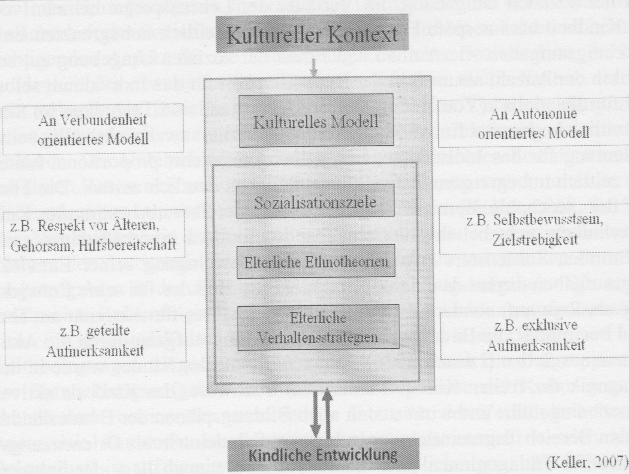
\includegraphics[width=0.85\textwidth]{grafik/kultur.png}
      \captionof{figure}[Zusammenwirken kultureller Kontexte und kindlicher Entwickung]{Zusammenwirken kultureller Kontexte und kindlicher Entwickung \citep[vgl.][S.~46]{Empirisch2012}}
      \label{fig:dittrich}
    \end{center}

    \begin{flushleft}
      Diese Grafik zeigt sehr anschaulich die Einbettung der kindlichen Entwicklung, zu der auch die Identit�tsentwicklung geh�rt, in den jeweiligen kulturellen Kontext. Rechts stehen die Faktoren von Erziehungsvorstellungen in kollektivistisch gepr�gten Kulturen und links die Faktoren in eher individualistisch gepr�gten Kulturen. Afrodeutsche Kinder erleben h�ufig beide Formen in der gleichen Familie. Auf diesen Punkt wird in Abschnitt \ref{sec:3_3_3} noch genauer eingegangen. Wichtig f�r einen kulturellen Kompetenzerwerb ist f�r Ruhs (2009), dass das Kind aus einer binationalen Familie ein \enquote{und} statt ein \enquote{oder} erf�hrt. Dass es aus beiden Kulturen, dass f�r ihn Wichtige mitnehmen kann, ohne sich entscheiden zu m�ssen. Insofern ist es auch wichtig, dass das Kind zu beiden Kulturen eine positive Einstellung hat. Hier wird die Aufgabe der Eltern angesprochen, ihren Kindern einen positiven Zugang zu beiden Kulturen zu gew�hren. Im Folgenden wird nun auf die Erfahrungswelten afrodeutscher Kinder im gesellschaftlichen Rahmen eingegangen, die einen nicht unerheblichen Einfluss auf ihre Identit�tsentwicklung haben. Dann folgt die Analysierung der famili�ren Situation afrodeutscher Kinder.
    \end{flushleft}


\newpage

\chapter{Lebenswirklichkeit von Afrodeutschen}\label{sec:3}
  \section{Afrodeutsch (Shirin Bediako)}\label{sec:3_1}
    \begin{flushleft}
    \end{flushleft}

    % \begin{center}
    %   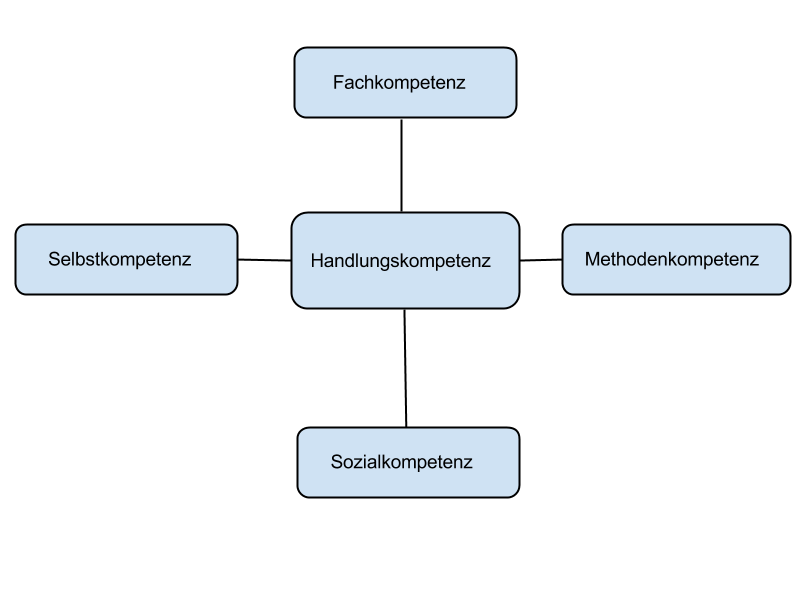
\includegraphics[width=0.85\textwidth]{grafik/taetigkeitspr.png}
    %   \captionof{figure}[Vierdimensionales Kompetenzmodell]{Vierdimensionales Kompetenzmodell \citep[vgl.][S.~15]{Kompet2011}}
    %   \label{fig:zusammenhang}
    % \end{center}

    \begin{flushleft}
    \end{flushleft}


  \section{Schwarzsein, Wei�sein - Deutschsein  (Shirin Bediako)}\label{sec:3_2}
    \begin{flushleft}
    \end{flushleft}

    \begin{flushleft}
    \end{flushleft}

    \begin{flushleft}
    \end{flushleft}


  \section{Mono- und Bikulturelle Familienstrukturen und Erziehungsstile (Shirin Bediako)}\label{sec:3_3}
    \begin{flushleft}
    \end{flushleft}

    \subsection{Deutsche Familien}\label{sec:3_3_1}
      \begin{flushleft}
      \end{flushleft}
      
    \subsection{Westafrikanische Familien}\label{sec:3_3_2}
      \begin{flushleft}
      \end{flushleft}
    
    \subsection{Westafrikanisch-deutsche Familien}\label{sec:3_3_3}
      \begin{flushleft}
      \end{flushleft}
      




    % \begin{flushleft}
    %   Eine Spielanalyse kann wie folgt aussehen:
    %   \begin{itemize}
    %     \item Inwieweit werden Kinder dazu ermutigt in diesem Spiel empathisch zu sein?
    %     \item Inwieweit werden verschiedene Rollen in diesem Spiel eingenommen und ausgehandelt?
    %     \item Wie sieht in diesem Spiel die Kontaktaufnahme unter den Kindern aus?
    %     \item Inwiefern ist es f�r dieses Spiel von N�ten, sich gegenseitig zu helfen und mit anderen zu kooperieren?
    %     \item Welche Regeln gibt es und m�ssen diese gegebenfalls mit den Kindern abgesprochen bzw. neu definiert werden?
    %   \end{itemize}
    % \end{flushleft}

\newpage

\chapter{Bikulturelle Identitätsentwicklung afrodeutscher Kinder}\label{sec:4}
  \section{\enquote{Doppeltes Anderssein} -  Zugehörigkeitsgefühl afro-deutscher Kinder (Shirin Bediako)}\label{sec:4_1}
    \begin{flushleft}
    \end{flushleft}

    \begin{flushleft}
    \end{flushleft}


  \section{Identitätsmuster nach Wießmeier als Umgangsweisen (Jelker Drücker)}\label{sec:4_2}
    \begin{flushleft}
    \end{flushleft}

    \begin{flushleft}
    \end{flushleft}

  
  \section{Bildung einer Patchworkidentität als mögliche Lösung (Jelker Drücker)}\label{sec:4_3}
    \begin{flushleft}
    \end{flushleft}

  \section{Bikulturalität als Chance (Jelker Drücker)}\label{sec:4_4}
    \begin{flushleft}
    \end{flushleft}

\newpage


%---------------------------------------------------------------------------------------------------
% Der dritte Teil der Arbeit
%---------------------------------------------------------------------------------------------------
\typeout{===== File: ZUSAMMENFASSUNG}
%---------------------------------------------------------------------------------------------------
% Zusammenfassung
%---------------------------------------------------------------------------------------------------
% \newpage
%%\part{Schluss}
\chapter{Res�mee}
  \section{Reflexion: Die Wichtigkeit von Studieninhalten f�r die Arbeit als Kita-Leitungskraft}
    \begin{flushleft}
      Die Verwendung eines Interviews und das drauf folgende Shadowing stellten sich als gute Methoden heraus, um das T�tigkeitsprofil einer Kita-Leitungskraft erforschen zu k�nnen. Besonders wichtig war mir zu erfahren, inwieweit die Studieninhalte des Bachelor Studienganges Bildung und Erziehung in der Kindheit auf die vielf�ltige und anspruchsvolle Arbeit einer Kita-Leitungskraft vorbereitet.
    \end{flushleft}

    \begin{flushleft}
      So konnte ich durch das Interview in Erfahrung bringen, dass sein eigenes Studium- Diplom Psychologie- inhaltlich f�r Herrn Strau� und seine Arbeit nicht so hilfreich war, wie er es sich erhofft hatte. Doch die praktischen Anwendungsgebiete wiederum haben ihn sehr geholfen, um vielen allt�glichen Gegebenheiten ad�quat begegnen zu k�nnen. Gerade das Selbststudium haben ihm Selbstst�ndigkeit, Analysef�higkeiten, Organisationsf�higkeiten und probleml�sungsorientiertes Handeln gelehrt. Auch ich bin der Meinung, dass das Selbststudium uns in vielerlei Hinsicht F�higkeiten und Fertigkeiten vermittelt, die f�r den Beruf der Leitungskraft sehr hilfreich sind. Wohingegen ich beim inhaltlichen Teil des Studiums nicht mit Herrn Strau� konform gehe. Den Ergebnissen der angewandten Methoden konnte ich ableiten, dass der ganze Managementsektor w�hrend des Studiums von Herrn Strau� eher stiefm�tterlich behandelt wurde und er sich sein Wissen durch Erfahrungen aneignen musst. Da dieser Teil der Arbeit aber in den letzten Jahren immer mehr an Bedeutung gewonnen hat, sieht er sich gezwungen eine Weiterbildung im Bereich Management zu machen. Diesem wurde im Studiengang Bildung und Erziehung in der Kindheit vorgebeugt, indem Studierende dieses Studienganges durch das Hauptfach Management mit diesem Bereich schon in Ber�hrung kommen. Auch Seminare wie Selbst- oder Beratungskompetenz vermitteln theoretisches Wissen, das f�r den praktischen Alltag hilfreich sein kann.
    \end{flushleft}

    \begin{flushleft}
      Ich m�chte jetzt aber auch nicht ohne weiteres behaupten, dass alle Studieninhalte Relevanz f�r den Leitungsberuf haben. Des Weiteren bin ich der Meinung, dass viele Inhalte im Studium bzw. in Vorlesungen und Seminaren nur angerissen werden und ich bei einem weiterf�hrenden Interesse an einem bestimmten Thema, auf das Selbststudium zur�ck greifen muss. 
    \end{flushleft}

    \begin{flushleft}
      Schlussendlich w�rde ich behaupten, dass das Studium uns vielerlei Mittel und Informationen mitgibt die wir selbst zu b�ndeln und eigenverantwortlich weiterzuf�hren haben. Dies sollte als gute Schule f�r die sp�tere Berufswelt gesehen werden. Denn auch hier m�ssen wir lernen, unser theoretisches Wissen im Praxisalltag richtig  anzuwenden.
    \end{flushleft}

  \section{Fazit}
    \begin{flushleft}
      Die Zielsetzung dieser Arbeit war es, das T�tigkeitsprofil einer Kita-Leitungskraft zu beleuchten. Dies wurde an Hand von Herrn Strau�, der die Leitungsposition in der Kindertagesst�tte �bernimmt, gemacht. Zu diesem Zweck wurde erst gekl�rt, wie das Arbeits- und der Aufgabenbereich einer Kita-Leitung aussieht. Im weiteren Verlauf wurde dann darauf eingegangen, welchen gesetzlichen Rahmen, auf Bundes- wie auch auf Landesebene, zu beachten sind, um eine Kita leiten zu k�nnen. Dem folgte die Darlegung der Ergebnisse, die in Folge des Interviews und des Shadowings erlangt wurden. Zudem wurde er�rtert wie die zentralen Kompetenzbereiche dieses T�tigkeitfelds aussehen. Anhand der sich aus dem Interview und Shadowing erschlie�enden Erkenntnisse, wurde noch beleuchtet, welche organisationale Managementdimensionen als Kita-Leitung zu erf�llen sind. Abschlie�end wurde reflektiert, inwieweit das Interview und Shadowing Erkenntnisse erbracht haben, welche Relevanz das Studium f�r die Leitungst�tigkeit hat. 
    \end{flushleft}

    \begin{flushleft}
      Durch die Hausarbeit konnte gezeigt werden, wie vielf�ltig und anspruchsvoll die T�tigkeiten einer Leitungskraft sind. Zudem konnte man sehen, dass die p�dagogische Arbeit mit Kindern kaum bis gar nicht mehr zum T�tigkeitsfeld geh�rt. Daher ist es auch nicht verwunderlich, dass eine Kita-Leitungskraft �ber umfangreiche Kompetenzen verf�gen muss. Diese braucht sie haupts�chlich, um den Kita-Alltag mit all seinen Facetten zu begegnen, organisieren und managen k�nnen.
    \end{flushleft}

    \begin{flushleft}
      Nun zu meinem pers�nlichen Fazit. Ich hatte mir von dieser Facharbeit erhofft, zwei Sachen zu erfahren. Zum einen war es mir wichtig zu erfahren, welchen Stellenwert das Studium f�r die Arbeit einer Leitungskraft hat. Zum anderen wollte ich wissen, wie der Alltag und die Aufgaben einer Leitungskraft aussehen, da ich selbst bis jetzt nur Erfahrungen in der p�dagogischen Arbeit am Kind gemacht habe. 
    \end{flushleft}

    \begin{flushleft}
      Durch die angewandten Methoden und Instrumente konnte ich beide Ziele zu meiner vollsten Zufriedenheit erf�llen. Ich hatte im Rahmen dieser Arbeit die Gelegenheit, viele Erkenntnisse �ber den Alltag und die Aufgaben eine Kita-Leitungskraft  zu erlangen. Des Weiteren konnte ich durch die Analyse und Reflexion der Ergebnisse sehr gut f�r mich herausfiltern, welchen Stellenwert dieses Studium und ein Studium an sich f�r die Arbeit als Leitung einer Kindertagesst�tte hat. Diese neu gewonnen Erkenntnisse sind von gro�er Bedeutung f�r meine sp�tere Berufswahl. 
    \end{flushleft}

  \section{Ausblick}
    \begin{flushleft}
      Durch die im Rahmen dieser Hausarbeit durchgef�hrte Untersuchungen, konnte ich mir ein erstes Bild von dem T�tigkeitsfeld einer Kita-Leitungskraft machen. Da dieses Bild aber nur �ber einen sehr kurzen Zeitraum gebildet wurde und ich noch gerne mehr Praxisbezogenes �ber diesen Beruf erfahren w�rde, steht f�r mich fest, dass ich gerne im folgenden Semester ein Praktikum in diesen Bereich machen m�chte.  
    \end{flushleft}



%%%%

% \clearpage
\cleardoublepage
% \typeout{===== Section: Anhang}
% \appendix
% 
% \includepdfset{pagecommand={\pagestyle{scrheadings}}}
% \includepdf[pages=-, addtotoc={1,chapter,0,Interview mit Herrn Strau�,chap:anhang_1}, scale=0.90, offset=6mm -5mm]{Interview.pdf}
% 
% \includepdfset{pagecommand={\pagestyle{scrheadings}}}
% \includepdf[pages=-, addtotoc={1,chapter,0,Interviewleitfaden zur Erforschung des Berufsfeldes,chap:anhang_2}, scale=0.90, offset=6mm -5mm]{Interviewleifaden.pdf} 
% 
% \includepdfset{pagecommand={\pagestyle{scrheadings}}}
% \includepdf[pages=-, addtotoc={1,chapter,0,Das Shadowing,chap:anhang_3}, scale=0.90, offset=6mm -5mm]{Shadowing.pdf}
% 
% \includepdfset{pagecommand={\pagestyle{scrheadings}}}
% \includepdf[pages=-, addtotoc={1,chapter,0,Dienstplanberechnung,chap:anhang_4}, scale=0.80, offset=6mm -5mm]{anhang_4.pdf}
% 
% \includepdfset{pagecommand={\pagestyle{scrheadings}}}
% \includepdf[pages=-, addtotoc={1,chapter,0,Verfassung der KiTa,chap:anhang_5}, scale=0.80, offset=6mm -5mm]{anhang_5.pdf}
% 
% \includepdfset{pagecommand={\pagestyle{scrheadings}}}
% \includepdf[pages=-, addtotoc={1,chapter,0,Grundriss der KiTa,chap:anhang_6}, scale=0.80, offset=6mm -5mm]{anhang_6.pdf}
% 
% \includepdfset{pagecommand={\pagestyle{scrheadings}}}
% \includepdf[pages=-, addtotoc={1,chapter,0,Beobachtungsbogen,chap:anhang_7}, scale=0.80, offset=6mm -5mm]{anhang_7.pdf}
% 
% \includepdfset{pagecommand={\pagestyle{scrheadings}}}
% \includepdf[pages=-, addtotoc={1,chapter,0,Einzel Soziogramm,chap:anhang_8}, scale=0.80, offset=6mm -5mm]{anhang_8.pdf}
% 
% \includepdfset{pagecommand={\pagestyle{scrheadings}}}
% \includepdf[pages=-, addtotoc={1,chapter,0,Kinderfragebogen,chap:anhang_9}, scale=0.80, offset=6mm -5mm]{anhang_9.pdf}
% 
% \includepdfset{pagecommand={\pagestyle{scrheadings}}}
% \includepdf[pages=-, addtotoc={1,chapter,0,Meinungsbild Mittagessen,chap:anhang_10}, scale=0.80, offset=6mm -5mm]{anhang_10.pdf}

% bibliography and other stuff
\backmatter
% \pagenumbering{arabic}
\typeout{===== Section: Literaturverzeichnis}
\cleardoublepage  
\phantomsection
\addcontentsline{toc}{chapter}{Literaturverzeichnis}
\bibliographystyle{natdin}
\bibliography{literatur}

% \typeout{===== Section: Glossar}
% \renewcommand{\glossaryname}{Glossar}
% \cleardoublepage  
% \phantomsection
% \addcontentsline{toc}{chapter}{Glossar}
% \clearpage
% \printglossaries

%% index
% \typeout{===== Section: Index}
\cleardoublepage  
% \phantomsection
% \addcontentsline{toc}{chapter}{Index}
% \printindex






% \HAWasurency

\end{document}
